\documentclass{article}
\usepackage{amsmath, amssymb, amsthm, graphicx}
\usepackage{pgfplots, tikz, cancel, framed, hyperref}
\usepackage{mathrsfs, mdframed, enumitem}
% tlmgr install jknapltx rsfs zref needspace

\graphicspath{{./Images}}


% \geometry{margin=1in}
\usepackage[left=.75in, right=.75in, top=0.75in, bottom=1in]{geometry}
\pgfplotsset{compat=1.18}
\setlength{\parskip}{0.8em}
\setlength{\parindent}{0pt}

\newtheoremstyle{solution}
  {15pt}
  {15pt}
  {}
  {}
  {\bfseries}
  {: }
  { }
  {}

\theoremstyle{solution}
\newtheorem*{solution}{SOLUTION}

\newtheoremstyle{boldcaps}
  {15pt}
  {15pt}
  {}
  {0pt}
  {\bfseries}
  {: }
  {0.5em}
  {}

\theoremstyle{boldcaps}
\newtheorem{definition}{DEFINITION}

\newenvironment{boxeddefinition}
  {\begin{mdframed}\begin{definition}}
  {\end{definition}\end{mdframed}}

\theoremstyle{boldcaps}
\newtheorem{theorem}{THEOREM}[section]

\newenvironment{boxedtheorem}
  {\begin{mdframed}\begin{theorem}}
  {\end{theorem}\end{mdframed}}

\usetikzlibrary{calc,shapes}

\newcommand{\tikzmark}[1]{\tikz[overlay,remember picture] \node (#1) {};}
\pgfmathdeclarefunction{erf}{1}{%
  \pgfmathparse{(2/sqrt(pi))*((#1) - ((#1)^3)/3 + ((#1)^5)/10 - ((#1)^7)/42 + ((#1)^9)/216)}%
}


\pgfmathdeclarefunction{erfi}{1}{%
  \pgfmathparse{(2/sqrt(pi))*((#1) + ((#1)^3)/3 + ((#1)^5)/10 + ((#1)^7)/42 + ((#1)^9)/216)}%
}

\pgfplotsset{my style/.append style={axis x line=middle, axis y line=
middle, xlabel={$x$}, ylabel={$y$} }}

\DeclareMathOperator*{\argmax}{arg\,max}
% ------------------------------------------------------------

\title{E.C. - Math challenge \#1 \\ ENGR\& 204 \#17385}
\author{Brendan Tea}
\date{\today}

\begin{document}
\maketitle

\section{Problem 1.}

A trapezoid has consecutive sides of length $8$, $10$, and $12$ in that order. 
Find the largest possible area of such a trapezoid rounded down to the nearest integer.

\begin{definition}
    \textbf{AREA OF A TRAPEZOID}
    \begin{equation}
        A = \frac{a+b}{2}h
    \end{equation}
\end{definition}

\begin{solution}
When approaching an optimization problem, we are going to create an 
area function and evaluate the vertices. In this geometry problem, it 
important to realize that there are two possible variations on how we 
can create a trapezoid. 

% minipage side by side of Slant-Base-Slant vs. Base-Slant-Base
\begin{figure}[h]
            \centering
            \begin{minipage}[t]{0.48\textwidth}
                \vspace{0pt}
                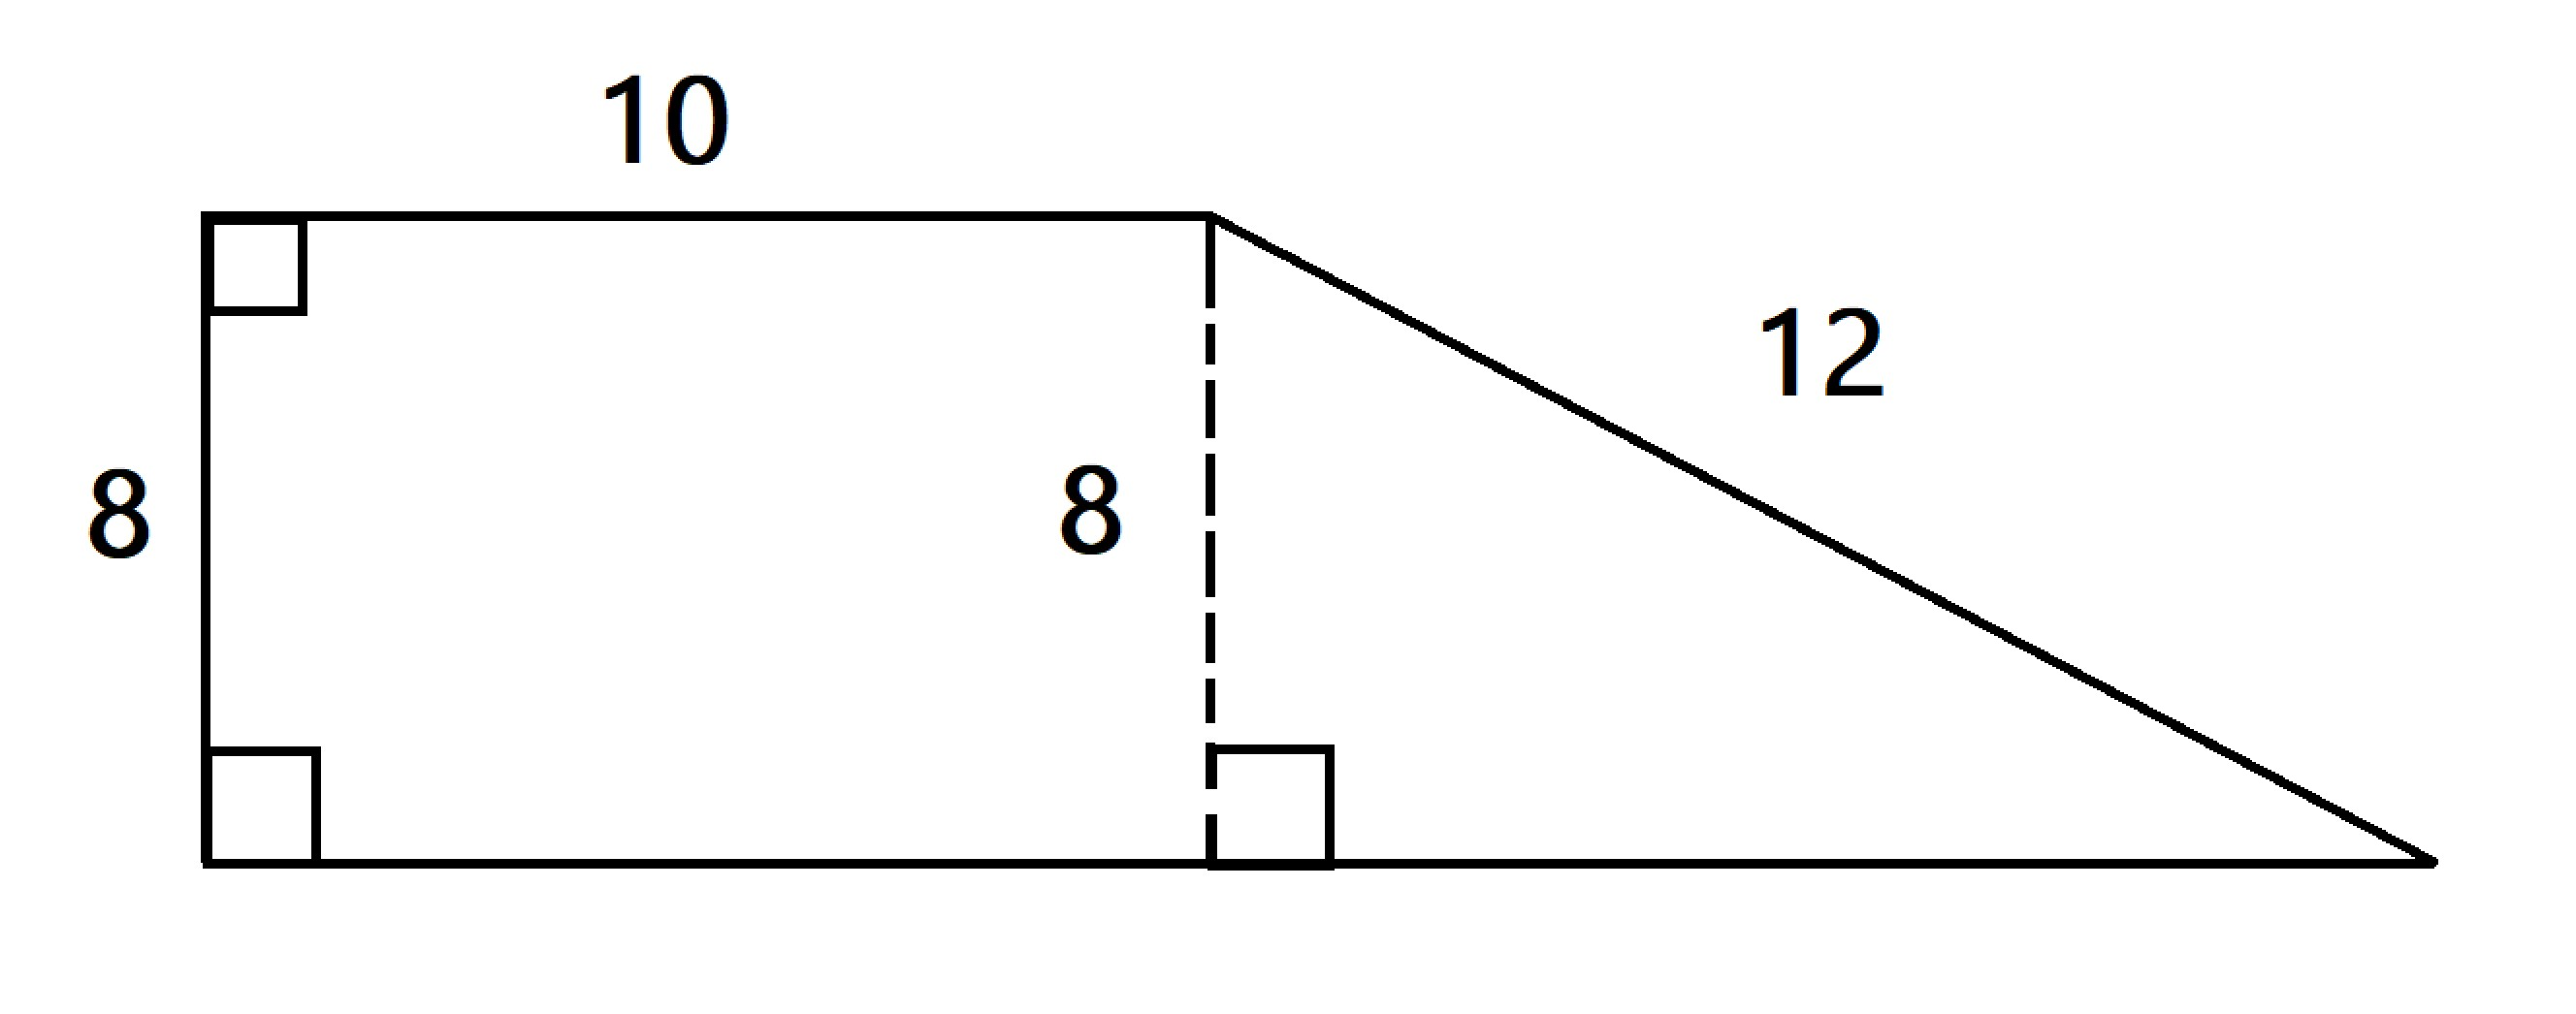
\includegraphics[width=1\linewidth]{maxheightsbs.jpg}
                \caption{Slant-Base-Slant Trapezoid}
            \end{minipage}
            \begin{minipage}[t]{0.48\textwidth}
                \vspace{0pt}
                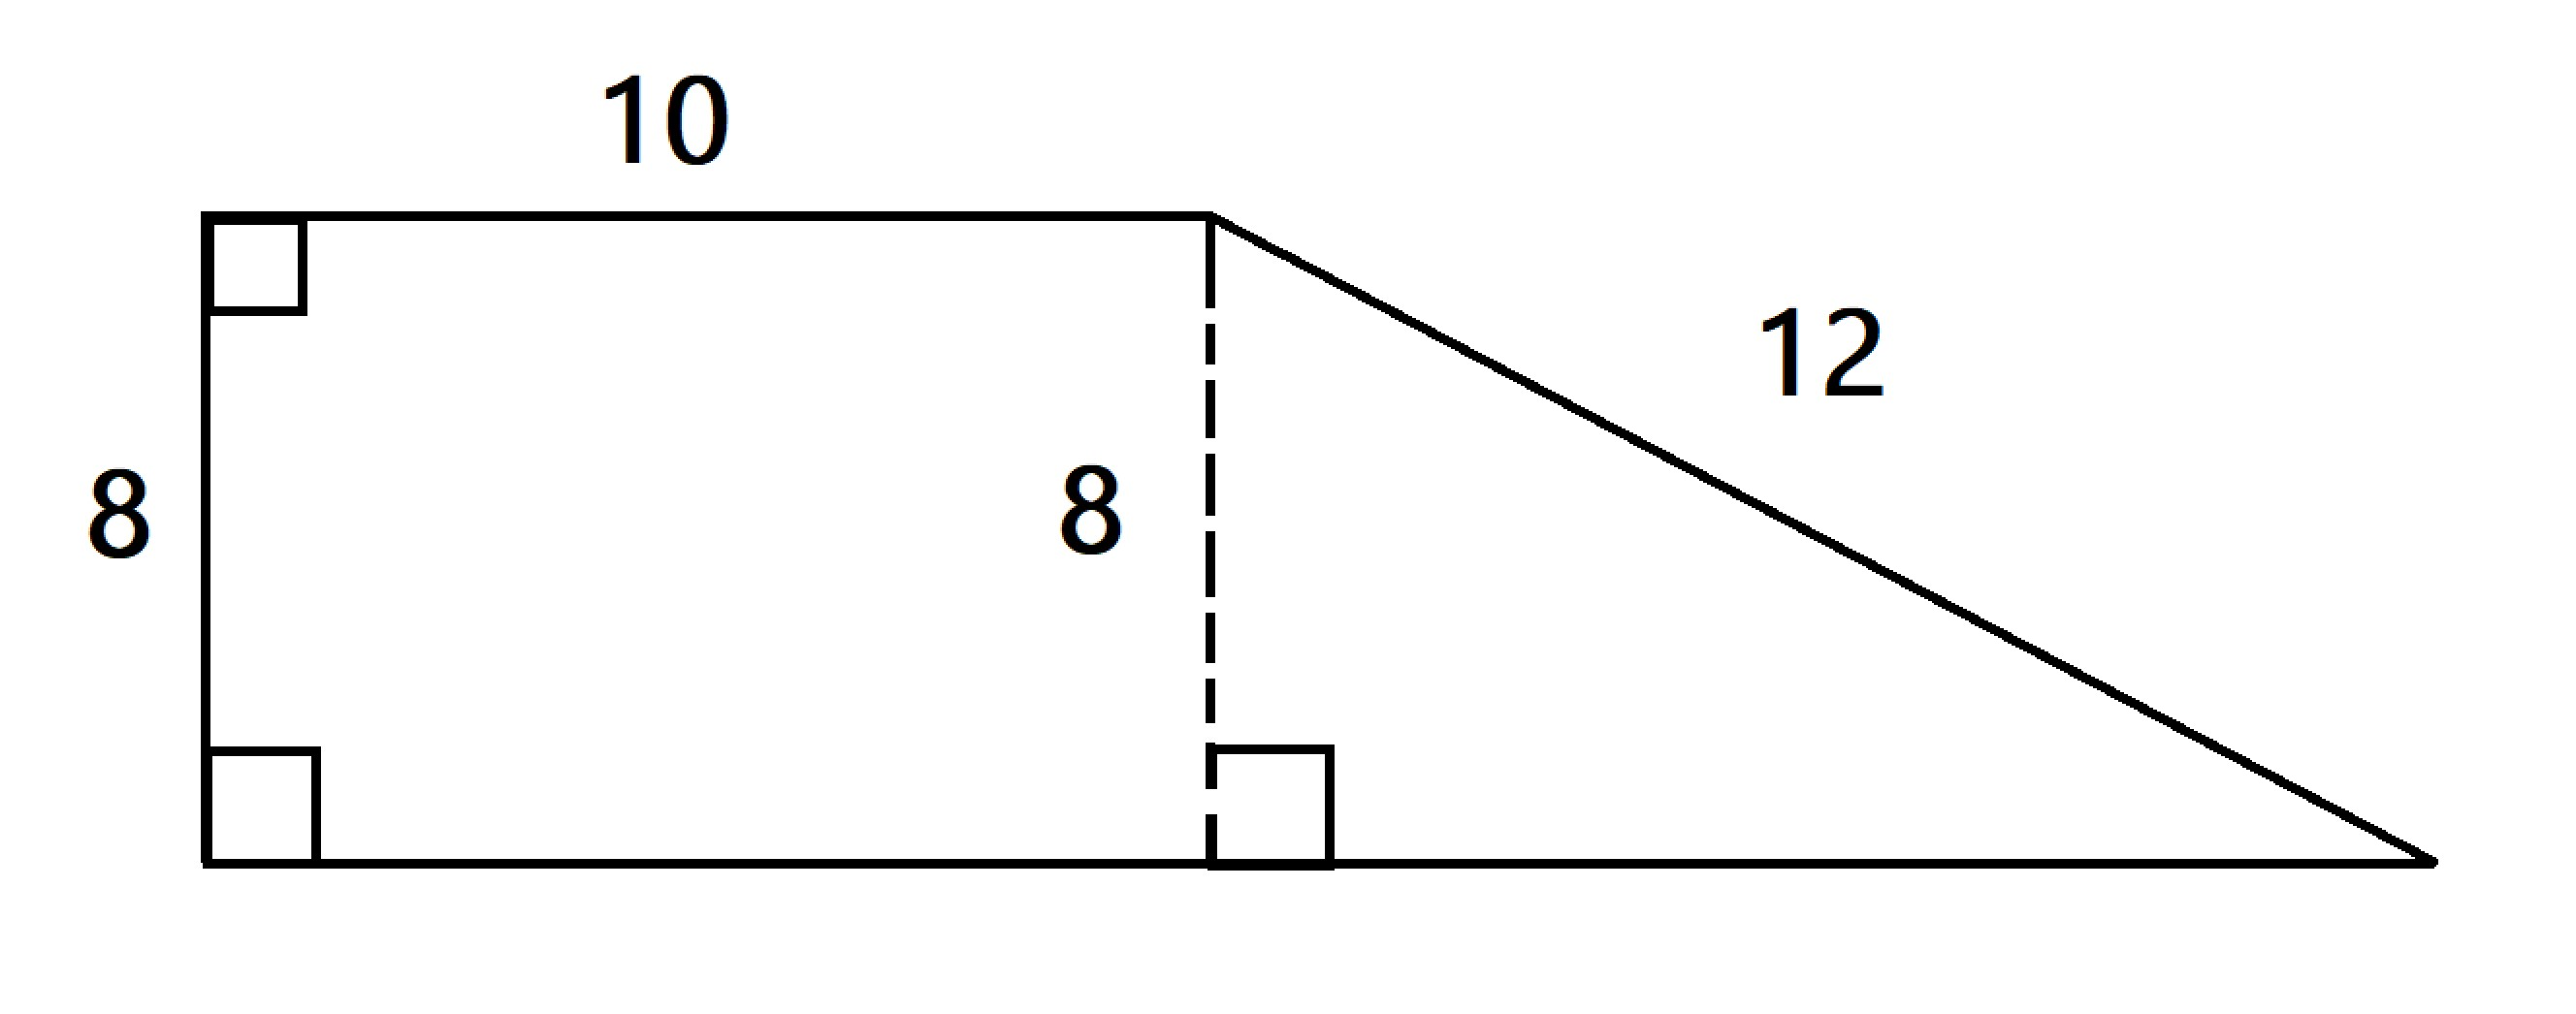
\includegraphics[width=1\linewidth]{maxheightsbs.jpg}
                \caption{Base-Slant-Base Trapezoid}
            \end{minipage}
        \end{figure}

We can either create a Slant-Base-Slant or a Base-Slant-Base trapezoid. Our
first problem is to decide whether each case gives out a larger area. Let us 
first start with the Base-Slant-Base case. Since we have fixed bases, we can simply
use our definition for area of a trapezoid. To maximize the area also implies 
maxing out the height if and only if the bases are fixed. More formally, we can
describe it with mathematical terms.

For a fixed $a, b \in \mathbb{R}^+$, it implies the following:
\begin{align*}
     A(h) &= \frac{a+b}{2}h \\
  \Longrightarrow   \argmax_{h} A &= \argmax_{h} h
\end{align*}

From this, we can logically find the maximum area for our Base-Slant-Base trapezoid
by making it a right trapezoid.
\begin{align*}
    a &= 8, \ b = 12, \ h = 10 \\
    A &= \frac{a+b}{2}h \\
    A_{bsb \ maxed}  &= \frac{8+12}{2}10 \\
\Longrightarrow    A_{bsb \ maxed} &= 100 \ \text{units}^{2}
\end{align*}

Our next case is the Slant-Base-Slant trapezoid. Something to note is that if we were 
to maximize height, we can show that the area of a Slant-Base-Slant trapezoid is larger than the 
area of a Base-Slant-Base trapezoid. This means that our answer is actually optimizing the 
Slant-Base-Slant triangle.

\begin{figure}[h]
    \centering
    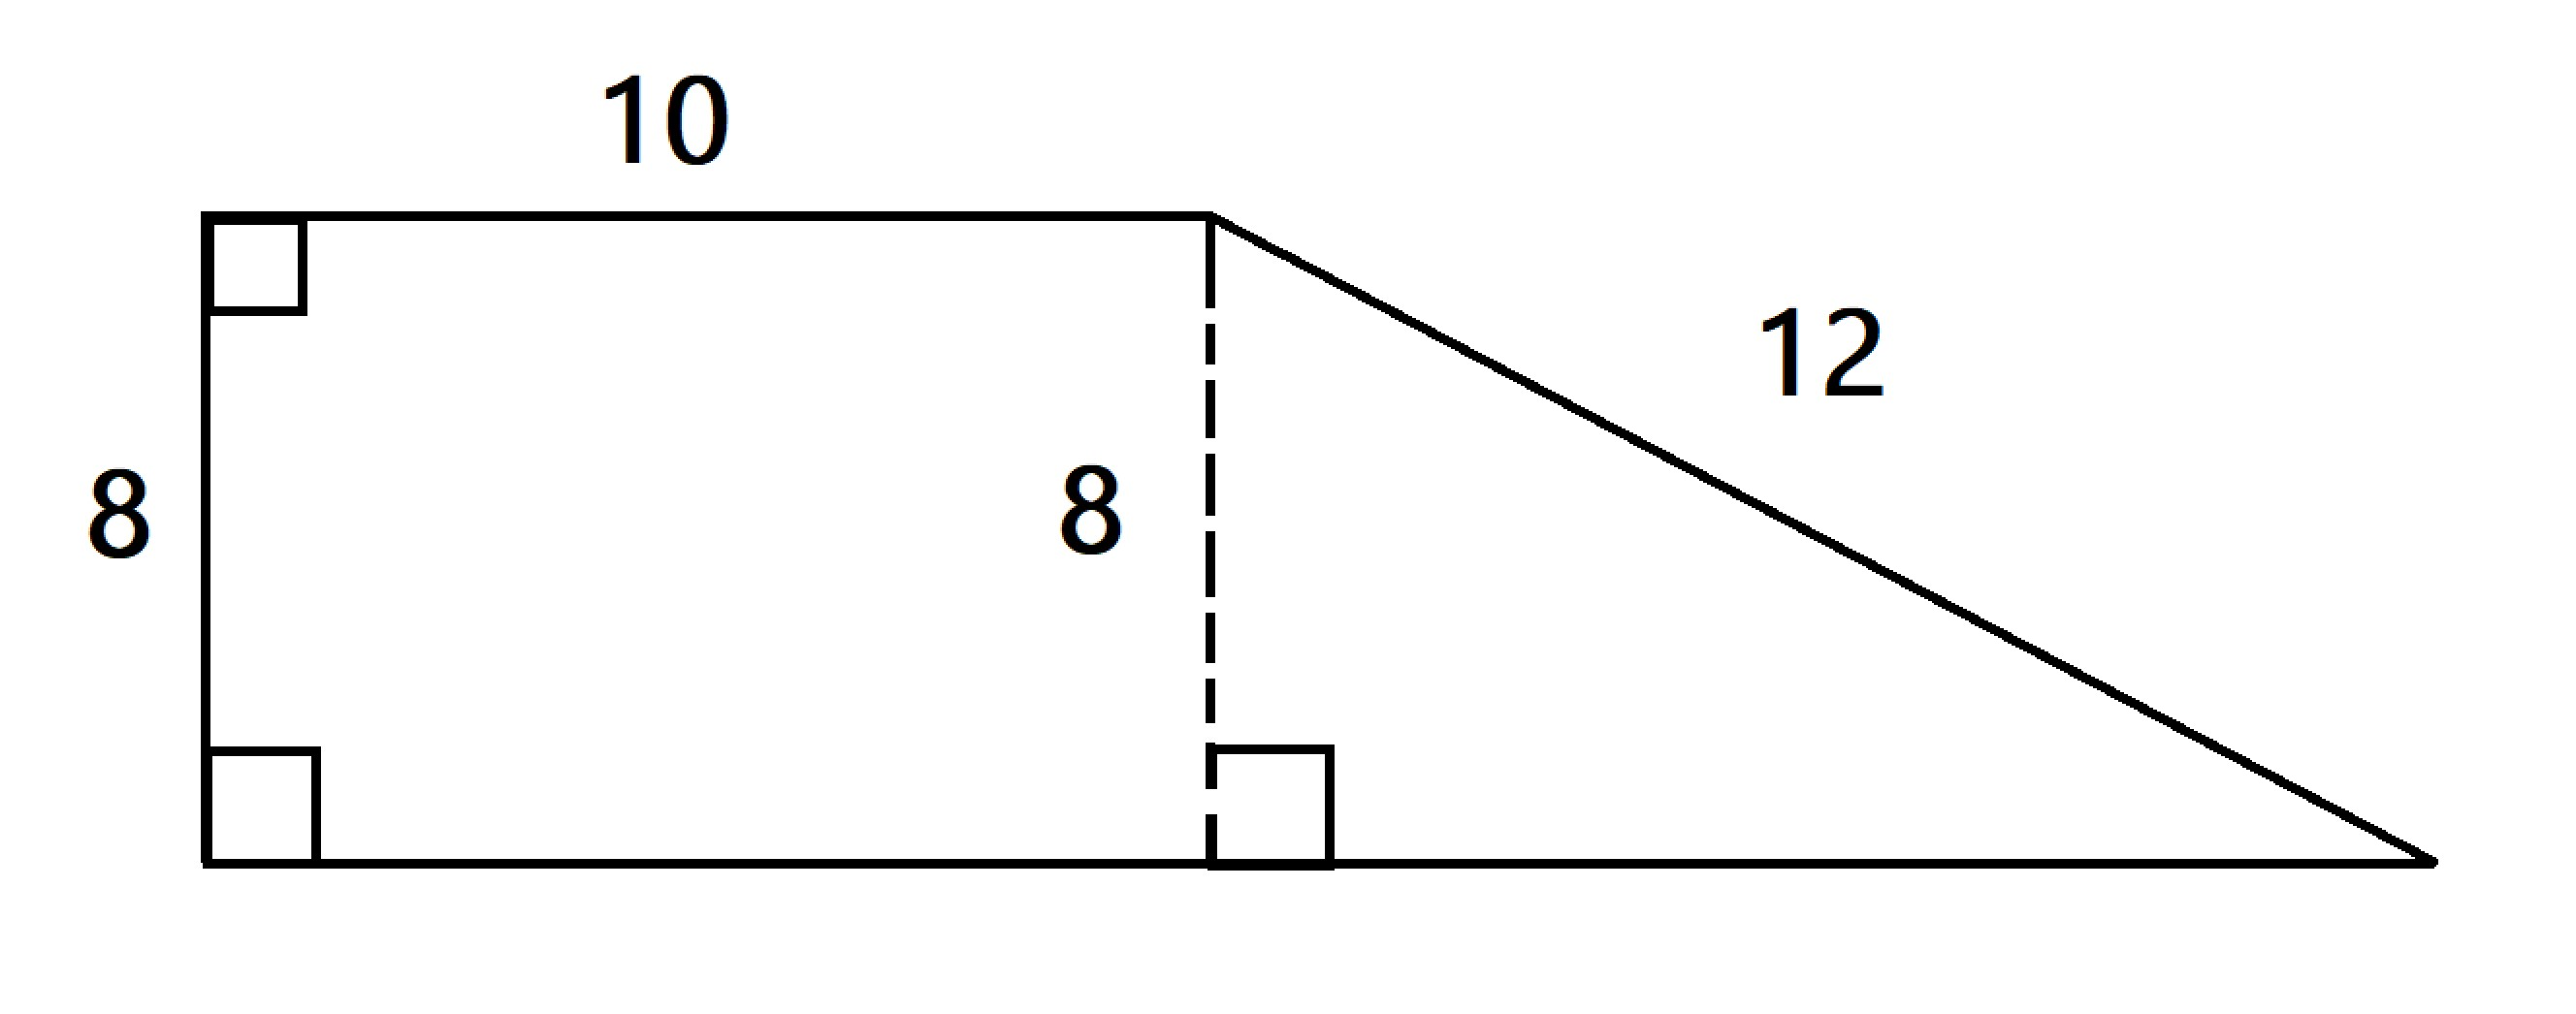
\includegraphics[width=0.4\linewidth]{maxheightsbs.jpg}
    \end{figure}
\begin{align*}
    s_{1} &= 8, \ a = 10, s_{2} = 12 \\
    A_{sbs} &= 8 \cdot 10 + \frac{8 \cdot (\sqrt{12^{2} - 8^{2}})}{2} \\
      &= 80 + 4 \sqrt{16 \cdot 5} \\
      &= 80 + 16 \sqrt{5} \\
    A_{sbs}  &\approx 115.777 \ \text{units}^{2} \\
    \Longrightarrow & \boxed{A_{sbs} > A_{bsb \ maxed}}
\end{align*}

\subsection{Optimizing Slant-Base-Slant Trapezoid}

\end{solution}
% %------------------------------------------------------%
% \include{Chapters/Section72.tex}
% %-------------------------------------------------%
% \include{Chapters/Section73.tex}

\end{document}